\textbf{Pré-requis:} Ce prototype ne prend pas en compte le \% de personnes utilisant les transports en communs.\\

Considérons trois centres de recherches et développements géographiquement très proches:
\begin{itemize}
\item L'école Polytech'Nice-Sophia
\item L'INRIA - Sophia Antipolis - Méditerranée , France
\item Le laboratoire i3s du CNRS \\
\end{itemize}

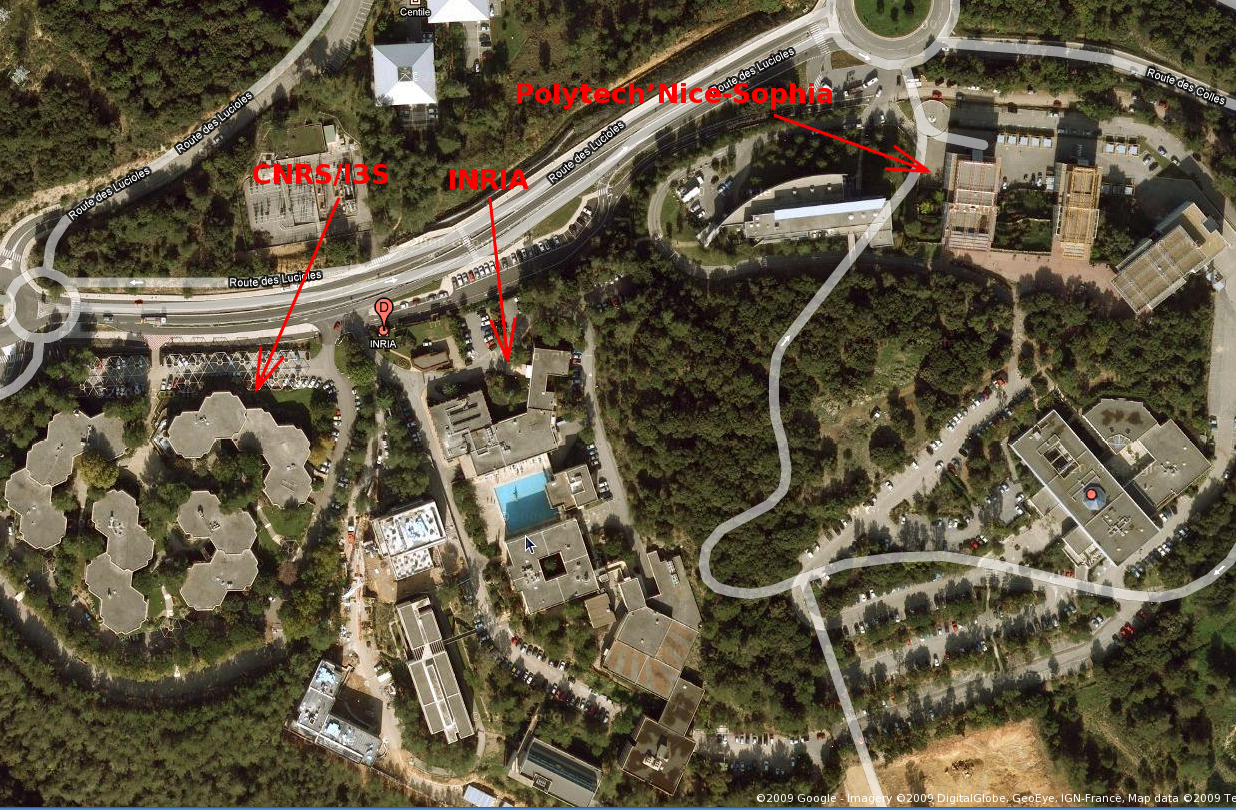
\includegraphics[scale=0.35]{img/screenshot/geolock} \\

Parmi ces 3 centres, on peut distinguer 2 types de personnes:
\begin{itemize}
\item Les Étudiants: \\
	Polytech'Nice-Sophia accueille près de \textbf{1.000 élèves} qui suivent les formations offertes dans cinq grands domaines scientifiques et technologiques  - Électronique, Informatique, Mathématiques appliquées, Génie biologique et Ingénierie de l'eau
\item Les Autres: \\
	Chercheurs, enseignants chercheurs, doctorant, ingénieurs, personnels administratifs, ...)
	repartis entre l'INRIA, le CNRS et l'école Polytech'Nice-Sophia (\textbf{environs 500 personnes}) \\
\end{itemize} 

Le cas critique pour cette zone géographique de sophia-antipolis, serai que toutes ces personnes possèdent une voiture sans jamais faire de covoiturage: environs 1500 voitures mobilisées tous les jours!
A l'inverse, le cas idéal serai que tout le monde propose de faire du co-voiturage, on obtiendrait pour 4 places disponibles par voiture:
1500/4 = 375 voitures mobilisées par jours, ce qui équivaut a une baisse de 75\% \\

Le but est donc ici d'optimiser au maximum le co-voiturage dans cette zone pour s'approcher le plus possible du cas idéal. 




